\appendix

\chapter{Captures d'écran de Redmine}
\label{annexe:redmine}

\begin{figure}[h]
	\centering
	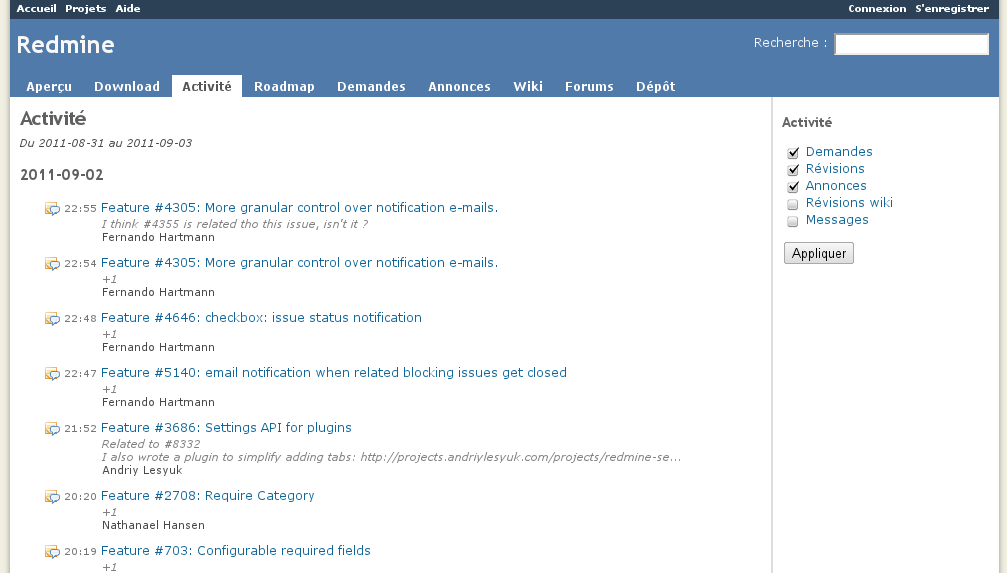
\includegraphics[width=14cm]{pic/redmine/activite}
	\caption{Redmine -- Onglet \og Activité \fg}
\end{figure}

\begin{figure}
	\centering
	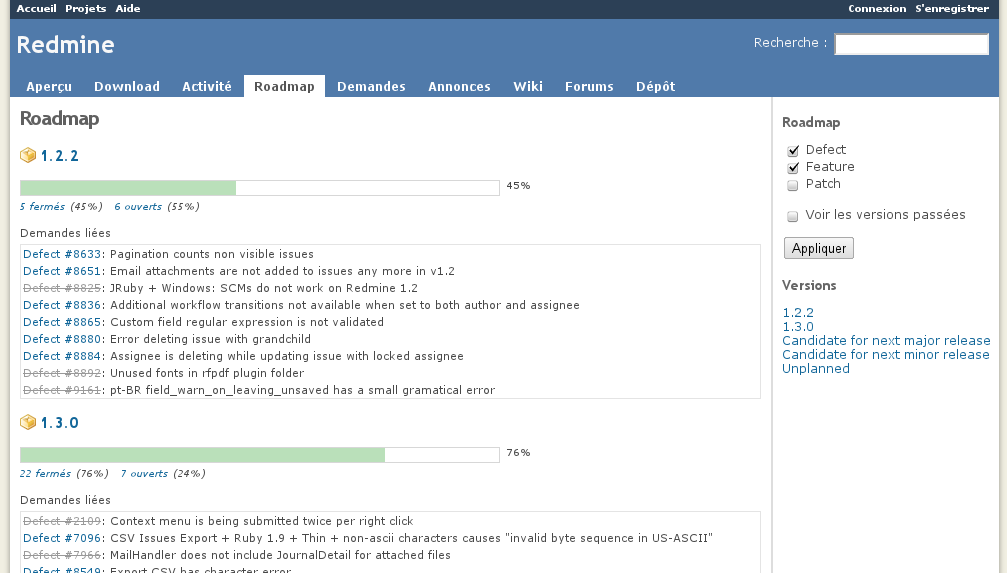
\includegraphics[width=14cm]{pic/redmine/roadmap}
	\caption{Redmine -- Onglet \og Roadmap \fg}
\end{figure}

\begin{figure}
	\centering
	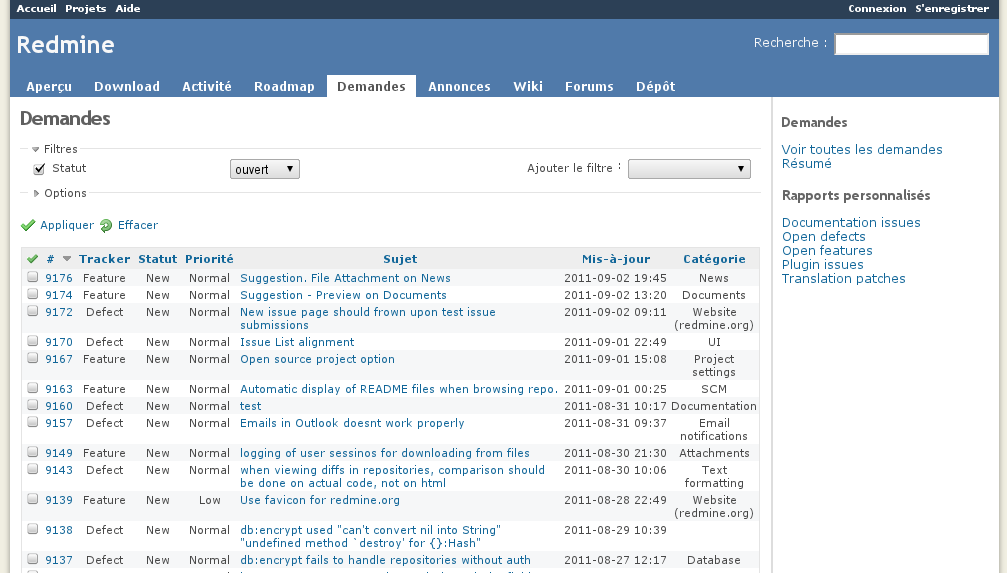
\includegraphics[width=14cm]{pic/redmine/liste-demandes}
	\caption{Redmine -- Onglet \og Demandes \fg}
\end{figure}

\begin{figure}
	\centering
	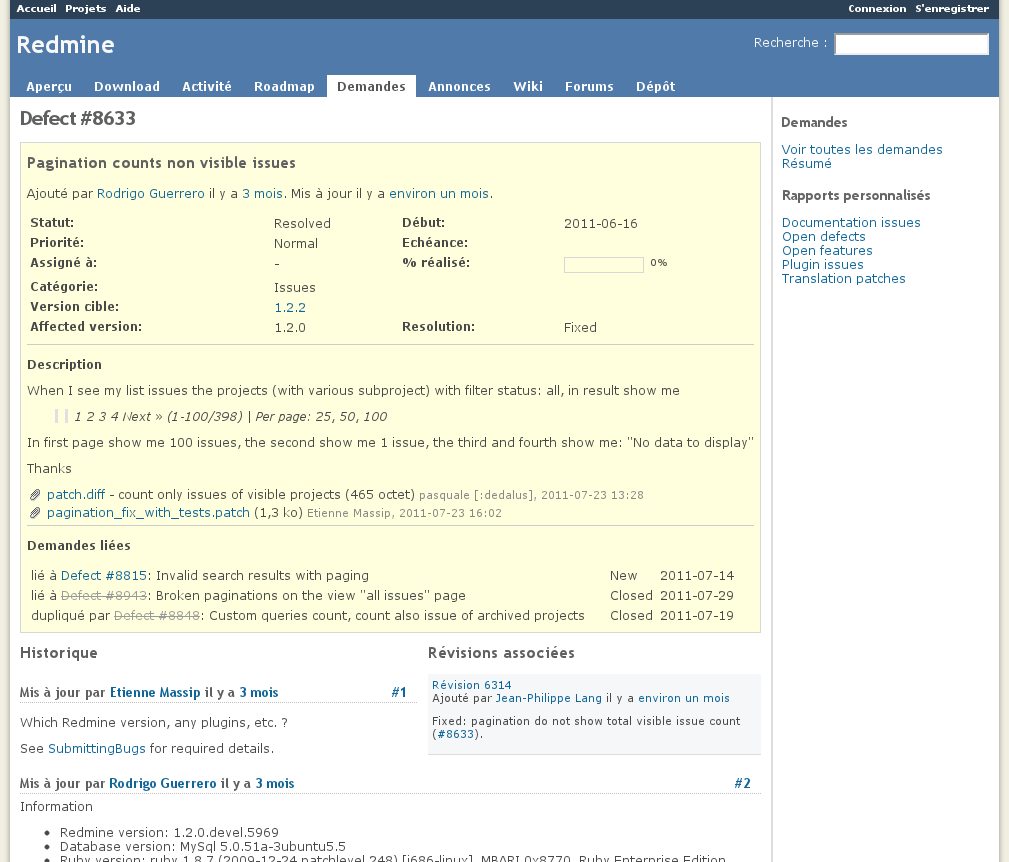
\includegraphics[width=14cm]{pic/redmine/demande}
	\caption{Redmine -- Détail d'une demande}
\end{figure}

\begin{figure}
	\centering
	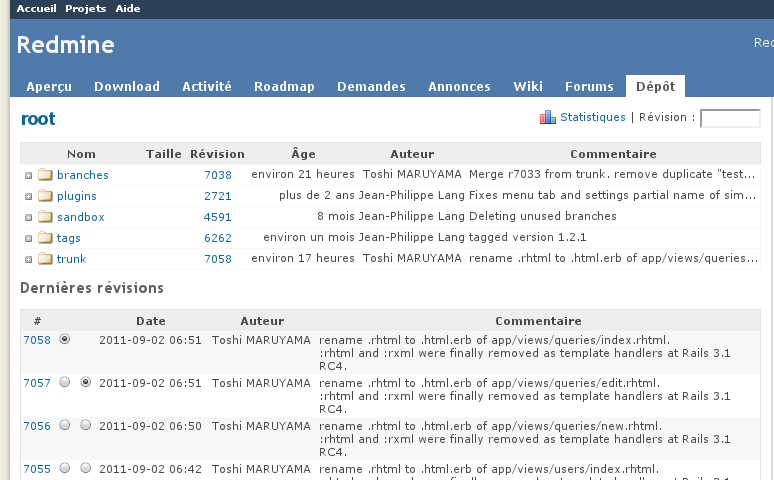
\includegraphics[width=10cm]{pic/redmine/depot}
	\caption{Redmine -- Onglet \og Dépôt \fg}
\end{figure}


\chapter{Captures d'écran de Jenkins}
\label{annexe:jenkins}

\begin{figure}[h]
	\centering
	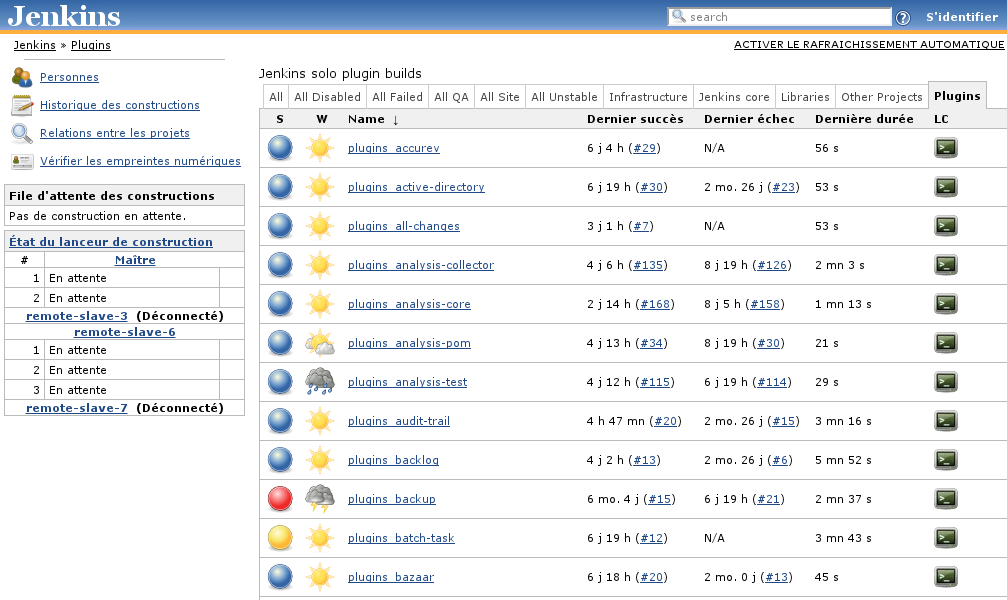
\includegraphics[width=14cm]{pic/jenkins/liste-projets}
	\caption{Jenkins -- Liste des projets}
\end{figure}

\begin{figure}
	\centering
	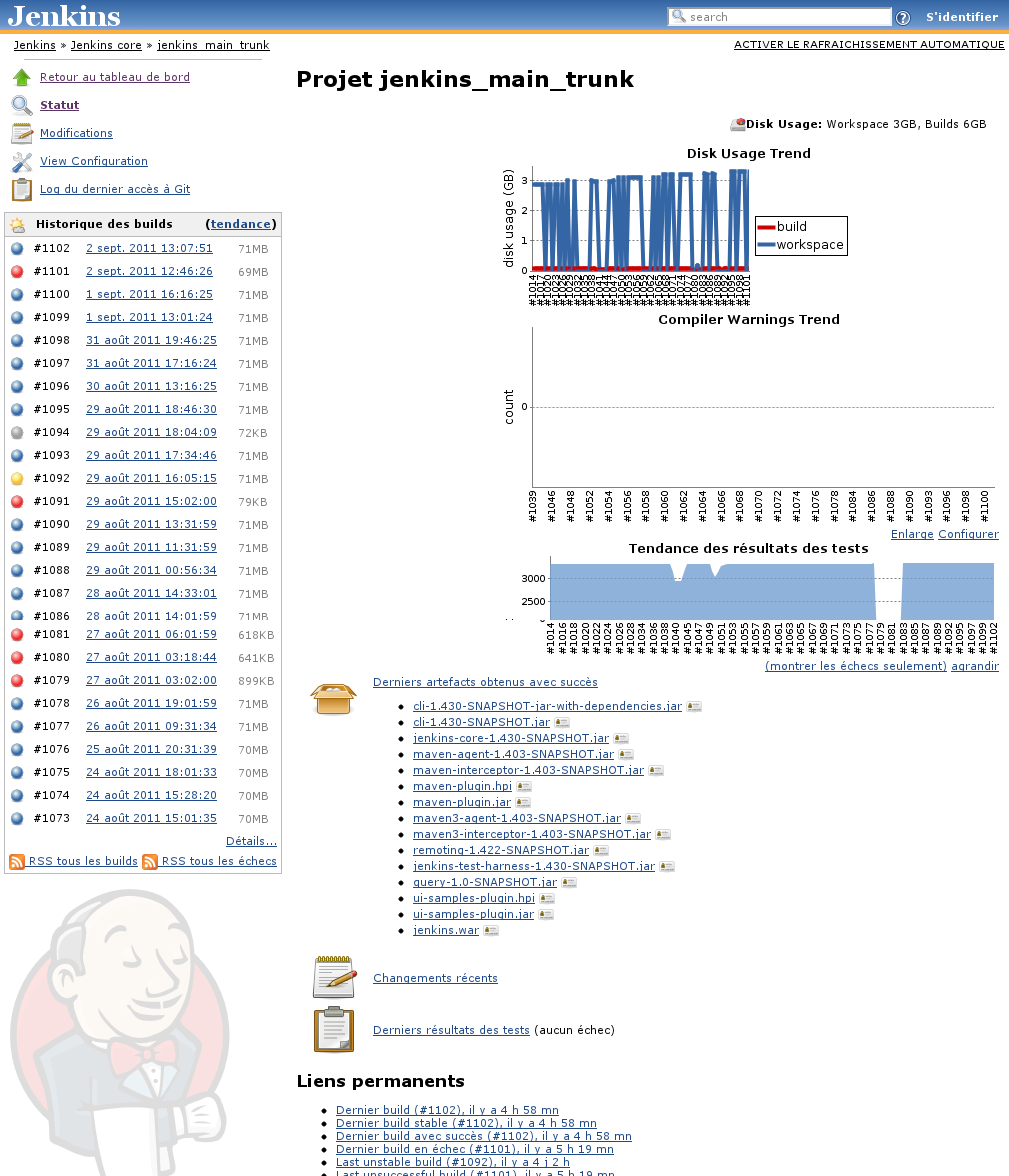
\includegraphics[width=14cm]{pic/jenkins/projet}
	\caption{Jenkins -- Tableau de bord d'un projet}
\end{figure}

\begin{figure}
	\centering
	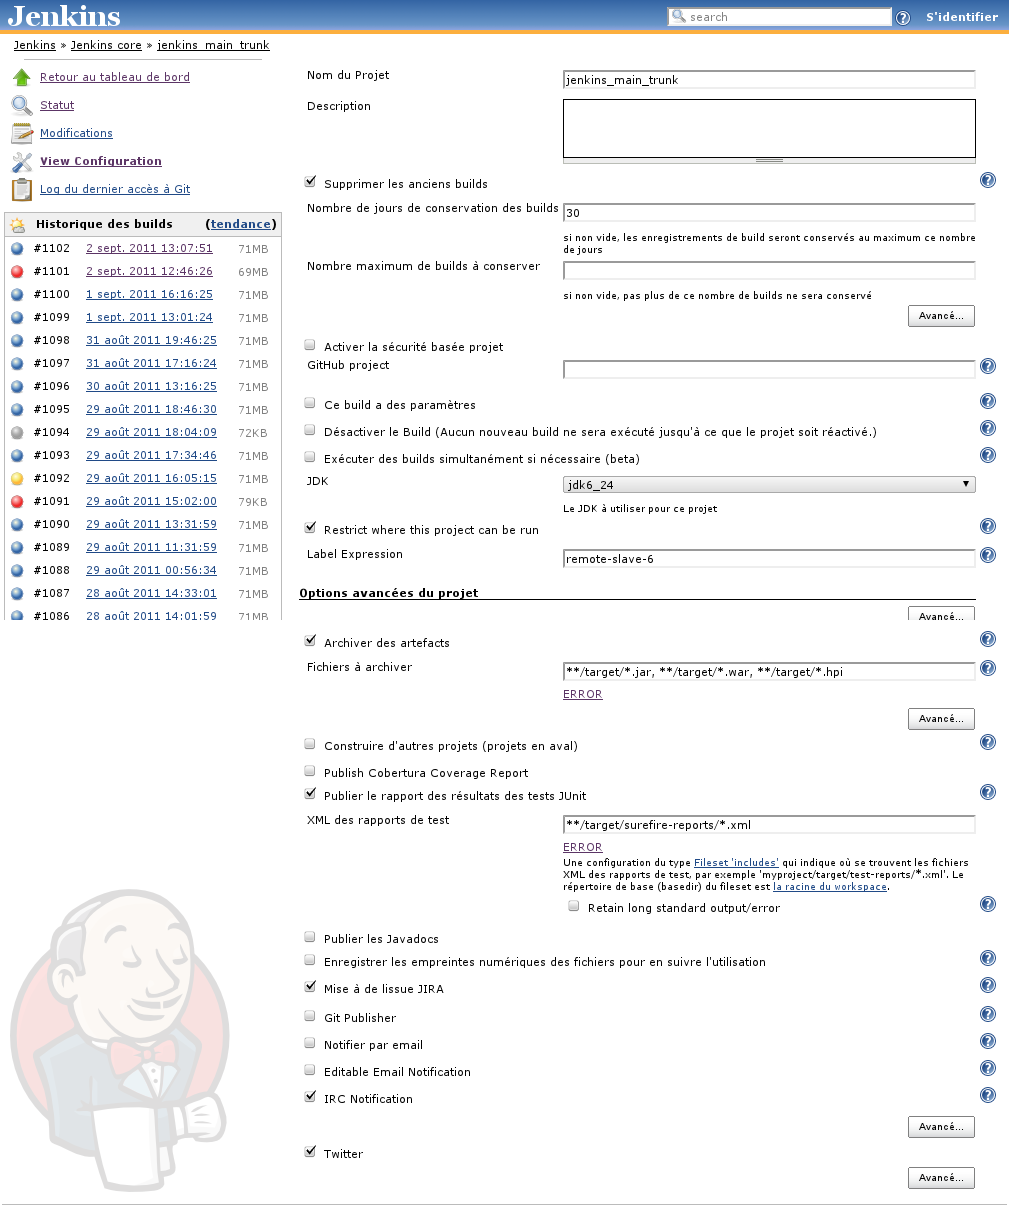
\includegraphics[width=14cm]{pic/jenkins/config}
	\caption{Jenkins -- Configuration d'un projet}
\end{figure}

